\subsubsection{BFS - Breadth First Search (Busca em largura)}
A busca em largura explora o grafo nível por nível, visitando primeiro todos os
vizinhos diretos de um nó antes de avançar para os vizinhos dos vizinhos. Para
isso, utiliza uma estrutura de dados de fila (\textit{Queue} - FIFO). Sua complexidade é: $\mathcal{O}(V+E)$

\paragraph{Pseudo-Código: }\mbox{}\\
\begin{algorithm}[H]
	%linhas dos blocos if, for
	\SetAlgoLined

	\SetKwFunction{BFS}{BFS}
	\SetKwProg{Fn}{Função}{:}{}

	\Fn{\BFS{$inicio, adj$}}{
		$fila \gets$ nova Fila()\;
		$visitado \gets$ novo vetor de booleanos\;
		$fila.push(inicio)$\;
		$visitado[inicio] \gets \text{true}$\;

		\While{\text{enquanto } $fila$ \text{ não vazia}}{
			$v \gets fila.front()$; $fila.pop()$\;
			\text{processar } $v$\;

			\ParaCada{$u \in adj[v]$}{
				\Se{$\neg visitado[u]$}{
					$visitado[u] \gets \text{true}$\;
					$fila.push(u)$\;
				}
			}
		}
	}
	\caption{Busca em Largura (BFS)}
\end{algorithm}

O funcionamento da BFS garante que encontramos o caminho mais curto em grafos
não ponderados, pois ela expande as frentes de busca de forma uniforme.

Veja a BFS funcionando de maneira mais visual, iniciando em $BFS(1)$:\\
\vspace{0.5cm} \noindent % Garante que não haja recuo de parágrafo indesejado
\begin{minipage}[t]{0.31\textwidth}
	\centering
	\textbf{Passo 1: Início}\\
	\vspace{0.2cm}
	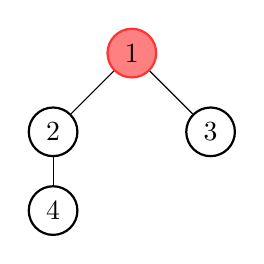
\begin{tikzpicture}[every node/.style={circle, draw, minimum size=0.5cm, thick},
			visited/.style={fill=gray!30},
			current/.style={fill=red!50, draw=red!80}]

		\node[current] (1) at (0, 1) {1};
		\node (2) at (-1, 0) {2};
		\node (3) at (1, 0) {3};
		\node (4) at (-1, -1) {4};

		\draw (1) -- (2);
		\draw (1) -- (3);
		\draw (2) -- (4);
	\end{tikzpicture}

	\vspace{0.2cm}
	\footnotesize
	\raggedright
	Insere 1 na fila. O nó 1 é o atual. Fila: [1].
\end{minipage}
\hfill
\begin{minipage}[t]{0.31\textwidth}
	\centering
	\textbf{Passo 2: Expandindo 1}\\
	\vspace{0.2cm}
	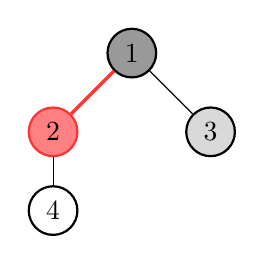
\begin{tikzpicture}[every node/.style={circle, draw, minimum size=0.5cm, thick},
			visited/.style={fill=gray!30},
			current/.style={fill=red!50, draw=red!80},
			finished/.style={fill=gray!80}]

		\node[finished] (1) at (0, 1) {1};
		\node[current] (2) at (-1, 0) {2};
		\node[visited] (3) at (1, 0) {3};
		\node (4) at (-1, -1) {4};

		\draw[very thick, red!80] (1) -- (2);
		\draw[visited] (1) -- (3);
		\draw (2) -- (4);
	\end{tikzpicture}

	\vspace{0.2cm}
	\footnotesize
	\raggedright
	Remove 1. Visita e insere os vizinhos 2 e 3 na fila. Fila: [2, 3].
\end{minipage}
\hfill
\begin{minipage}[t]{0.31\textwidth}
	\centering
	\textbf{Passo 3: Expandindo 2}\\
	\vspace{0.2cm}
	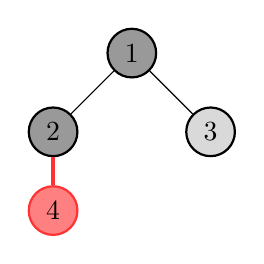
\begin{tikzpicture}[every node/.style={circle, draw, minimum size=0.5cm, thick},
			visited/.style={fill=gray!30},
			current/.style={fill=red!50, draw=red!80},
			finished/.style={fill=gray!80}]

		\node[finished] (1) at (0, 1) {1};
		\node[finished] (2) at (-1, 0) {2};
		\node[visited] (3) at (1, 0) {3};
		\node[current] (4) at (-1, -1) {4};

		\draw[finished] (1) -- (2);
		\draw[visited] (1) -- (3);
		\draw[very thick, red!80] (2) -- (4);
	\end{tikzpicture}

	\vspace{0.2cm}
	\footnotesize
	\raggedright
	Remove 2. Visita e insere o vizinho 4. Fila: [3, 4].
\end{minipage}
\vspace{0.3cm}
\noindent
\begin{center}
	\textbf{Passo 4: finalizando BFS}\\
	\vspace{0.2cm}
	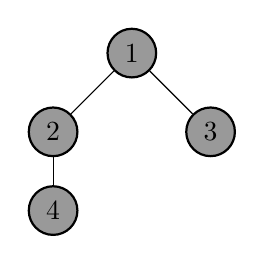
\begin{tikzpicture}[every node/.style={circle, draw, minimum size=0.5cm, thick},
			visited/.style={fill=gray!30},
			current/.style={fill=red!50, draw=red!80},
			finished/.style={fill=gray!80}]

		\node[finished] (1) at (0, 1) {1};
		\node[finished] (2) at (-1, 0) {2};
		\node[finished] (3) at (1, 0) {3};
		\node[finished] (4) at (-1, -1) {4};

		\draw[finished] (1) -- (2);
		\draw[finished] (1) -- (3);
		\draw[finished] (2) -- (4);
	\end{tikzpicture}

	\footnotesize
	\centering
	Removemos o vizinho 4 e ele não tinha vizinhos, então finalizado. E vamos remover 3 e vai ocorrer o mesmo de não ter vizinhos, logo finalizamos a BFS.
\end{center}
Veja que a ordem de visitação por níveis da BFS resulta em: $[1, 2, 3, 4]$.

\paragraph{Implementação: }\mbox{}
Vejamos a implementação da BFS em Python e em C++.

\textbf{Python: }
\begin{lstlisting}[language=Python]
	from collections import deque
	
	def bfs(inicio, adj):
	visitado = [False] * len(adj)
	fila = deque([inicio])
	visitado[inicio] = True
	
	while fila:
	v = fila.popleft()
	print(v) # Processa o vertice atual
	for u in adj[v]:
	if not visitado[u]:
	visitado[u] = True
	fila.append(u)
\end{lstlisting}

\vspace{0.3cm}
\textbf{C++:}
\begin{lstlisting}[language=C++]
	void bfs(int inicio, const vector<vector<int>>& adj) {
		vector<bool> visited(adj.size(), false);
		queue<int> q;
		
		q.push(inicio);
		visited[inicio] = true;
		
		while (!q.empty()) {
			int v = q.front();
			q.pop();
			// Processa o vertice atual aqui
			
			for (int u : adj[v]) {
				if (!visited[u]) {
					visited[u] = true;
					q.push(u);
				}
			}
		}
	}
\end{lstlisting}